\documentclass[tikz,border=10pt]{standalone}
\usepackage{amsmath}
\usetikzlibrary{arrows.meta, positioning, fit}

\begin{document}
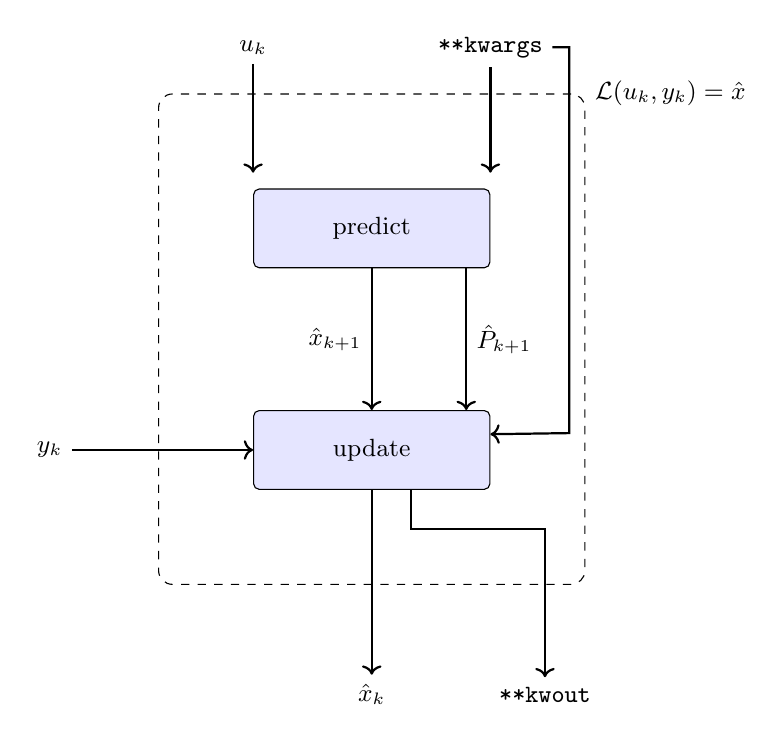
\begin{tikzpicture}[
  font=\small,
  box/.style={draw, rounded corners=2pt, minimum width=3cm, minimum height=1cm, fill=blue!10},
  arrow/.style={->, thick},
  dashedbox/.style={draw, dashed, rounded corners=5pt, inner sep=5pt},
]

% Internal blocks
\node[box] (predict) at (0,0) {predict};
\node[box, below=1.8cm of predict] (update) {update};

% Observer dashed box
\node[dashedbox, fit={(predict) (update)}, inner sep=1.2cm, label={[anchor=west]north east:$\mathcal{L}(u_k, y_k) = \hat{x}$}] (observerbox) {};

% External inputs
\node[above=2.3cm of predict.west, anchor=center] (uk) {$u_k$};
\node[above=2.3cm of predict.east, anchor=center] (kwargs) {\texttt{**kwargs}};
\node[left=2.3cm of update.west] (yk) {$y_k$};

% Outputs


% Arrows into predict
\draw[arrow] (uk) -- ([yshift=0.2cm]predict.north west);
\draw[arrow] (kwargs) -- ([yshift=0.2cm]predict.north east);

% Arrow from kwargs to update via elbow routing
\draw[arrow] (kwargs) -- ++(1.0,0) coordinate (r1) 
                        -- ++(0,-4.9) coordinate (r2)
                        -- ([yshift=0.2cm]update.east);




% Arrows from predict to update
\draw[arrow] (predict.south) -- node[left] {$\hat{x}_{k+1}$} (update.north);
\draw[arrow] ([xshift=1.2cm]predict.south) -- node[right] {$\hat{P}_{k+1}$} ([xshift=1.2cm]update.north);

% Arrow into update
\draw[arrow] (yk) -- (update.west);

% Output nodes
\node[below=2.6cm of update.south, anchor=center] (xhatk) {$\hat{x}_k$};
\node[below=2.6cm of update.south, xshift=2.2cm, anchor=center] (kwout) {\texttt{**kwout}};

% Output arrows
\draw[arrow] (update.south) -- ++(0,-0.5) -| (xhatk);
\draw[arrow] ([xshift=0.5cm]update.south) -- ++(0,-0.5) -| (kwout);

\end{tikzpicture}
\end{document}
